\begin{frame}[fragile]{Memory Objects: Buffers}
  \begin{lstlisting}[gobble=4]
    buf = cl.Buffer(context, flags, size=0, hostbuf=None)
  \end{lstlisting}
  \begin{columns}
    \column{0.7\textwidth}
      \begin{overlayarea}{\textwidth}{0.7\textheight}
        \only<+>{
          \begin{itemize}
            \item Chunk of device memory
            \item No type information: ``Bag of bytes''
            \item Observe: \emph{Not} tied to device.

              $\rightarrow$ no fixed memory address

              $\rightarrow$ pointers do \emph{not} survive kernel
              launches

              $\rightarrow$ movable between devices

              $\rightarrow$ not even allocated before first use!
            \item \texttt{flags}:
              \begin{itemize}
                \item \texttt{READ\_ONLY/WRITE\_ONLY/READ\_WRITE}
                \item \{\texttt{ALLOC,COPY,USE}\}\texttt{\_HOST\_PTR}
              \end{itemize}
          \end{itemize}
        }
        \only<+>{
          \texttt{COPY\_HOST\_PTR}:
          \begin{itemize}
            \item Use \texttt{hostbuf} as initial content of buffer
          \end{itemize}
          \texttt{USE\_HOST\_PTR}:
          \begin{itemize}
            \item \texttt{hostbuf} \emph{is} the buffer. 
            \item Caching in device memory is allowed.
          \end{itemize}
          \texttt{ALLOC\_HOST\_PTR}:
          \begin{itemize}
            \item \emph{New} host memory (unrelated to
              \texttt{hostbuf}) is visible from device
              \emph{and} host.
          \end{itemize}
        }
        \only<+>{
          \begin{itemize}
            \item Specify \texttt{hostbuf} or \texttt{size} (or both)
            \item \texttt{hostbuf}: Needs Python Buffer Interface\\
              e.g. \texttt{numpy.ndarray}, \texttt{str}.
              \subitem{Important: Memory layout matters}
            \item Passed to device code as pointers\\
              (e.g. \texttt{float *}, \texttt{int *})
            \item \texttt{enqueue\_copy}(queue, dest, src)
            \item Can be mapped into host address space:\\
              \texttt{cl.MemoryMap}.
          \end{itemize}
        }
      \end{overlayarea}
    \column{0.3\textwidth}
      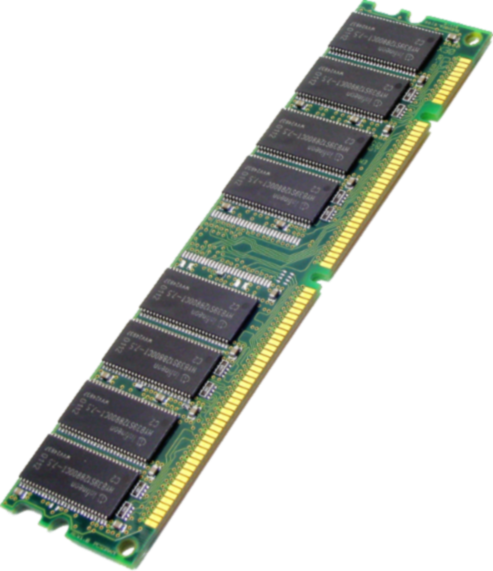
\includegraphics[width=\textwidth]{memory.png}
  \end{columns}
\end{frame}
\addimgcredit{RAM stick: sxc.hu/gobran11}
